\documentclass[12pt]{article}

%---------------------------------------------------------------------
% PACOTES PADRÕES (Não remover)
\usepackage{sbc-template}
\usepackage{graphicx,url}
\usepackage[german]{babel}   
\usepackage[utf8]{inputenc}  
\usepackage{verbatim}
\usepackage{listings}
\usepackage{indentfirst}
\usepackage{graphicx}
\usepackage{wrapfig}
\usepackage{amsmath}
\usepackage{amssymb}
\usepackage{float}




% PACOTES PESSOAIS (Insira abaixo seus pacotes utilizados)





%---------------------------------------------------------------------
\sloppy

% TÍTULO DO ARTIGO
\title{Lighthouse: Ein System zur effektiven Erkennung und Prävention von Corona Infektionsketten}

% AUTORES
\author{Mohammad Kohankhaki, Amanuel Aslan\inst{2}}

% E-MAILS
\address{m.kohankhaki@gmail.com \inst{2}manu.aslan77@gmail.com
}

%---------------------------------------------------------------------
\begin{document} 
\maketitle

\begin{abstract}
  Lighthouse ist ein zentralisiertes Infektionserkennungs- und Infektionspräventionsystem für das Corona Virus. Die Datensicherheit in Lighthouse wird durch asymmetrische Verschlüsselung und Anonymisierung gewährleitet. Es wird durch eine JAM-Stack Architektur realisiert und basiert somit auf einem Server-Client Modell, wobei Clients in Form von mobilen Anwendungen für Smartphones implementiert werden. Das System nutzt die Bluetooth Technologie auf Smartphones bzw. den Clients, um Kontakte zwischen Personen zu erkennen und mathematische Graphentheorie auf dem Backend bzw. Servern, um Infektionen zu erkennen und vorzubeugen. \\ \\
\end{abstract}

%---------------------------------------------------------------------
\section{Einführung}
\begin{wrapfigure}{R}{0.4\textwidth}
    \centering
    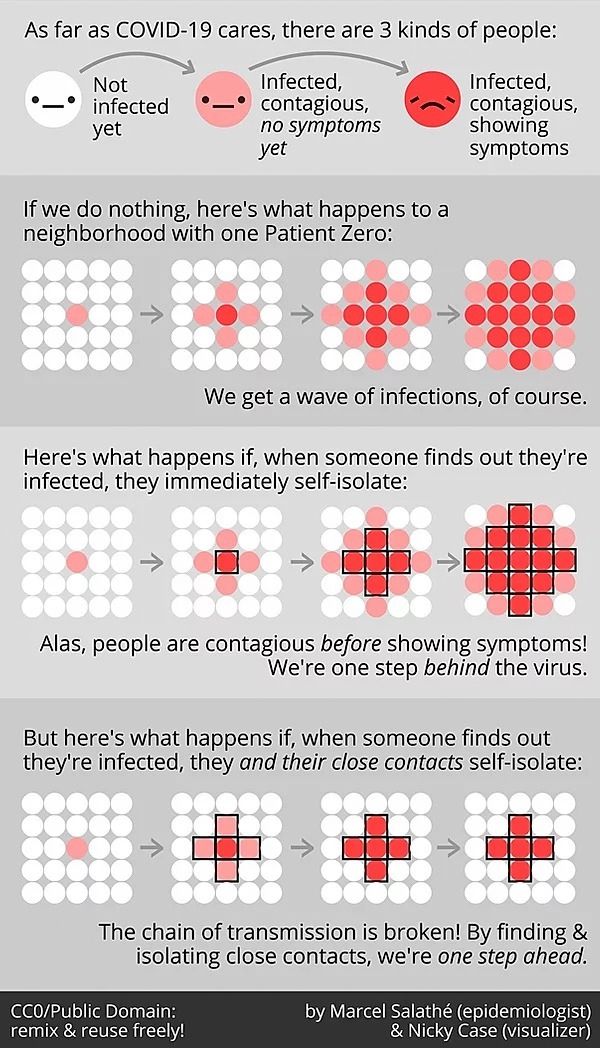
\includegraphics[width=0.35\textwidth]{res/infection_chain.jpeg}
    \caption{Infektionskette}
    \label{fig:inf_chain}
\end{wrapfigure}
Das Corona Virus breitet sich global wie ein Fegefeuer aus. Es gibt kaum eine Region auf dem Globus, die noch nicht vom unsichtbaren Feind heimgesucht wurde. Was das Virus so gefährlich macht ist die lange Inkubationszeit. Wie es auf der Abbildung \ref{fig:inf_chain} zu erkennen ist, ist die Erkennung von
bereits infizierten Personen wenig gewinnbringend für die Eindämmung der Pandemie. Die Hauptursache hierfür ist das Fehlen einer effektiven Methode zur Erkennung infizierter Personen bevor Symptome eintreten.
Während zwar Tests auf COVID-19 existieren, sind diese aufgrund
der genetischen Komplexität des Virus zeit- und ressourcenaufwendig, und
somit untauglich für die Massen. Was wir brauchen ist eine Erkennungsmethode, welche folgende Eigenschaften erfüllt:

\begin{itemize}
	\item \textbf{Realisierbarkeit}:  Massentauglichkeit und angemessener Zeit- und Ressourcenaufwand
	\item \textbf{Effektivität}: Signifikante Eindämmung der Infektionsrate
	\item \textbf{Genauigkeit}: Konformität zum gegenwärtigen Zustand
	\item (Daten)\textbf{Sicherheit}: Gefahrlosigkeit für Individuen
\end{itemize}


\section{Kontaktbasierte Erkennungssysteme}

Rund 81\% der Deutschen besitzen ein Smartphone (stand 2018). In Zeiten des IoT
ist das Smartphone bestimmt nicht der einzige tägliche Begleiter, jedoch ohne Zweifel der Wahrscheinlichste. Durch die Nutzung von Kurzwellentechnologien wie z.B. Bluetooth oder Wifi-Direct könnte man Kontakte zwischen Menschen erkennen und zusammen mit dem Datum des Kontakts speichern. Auf diese Art können wir ein Kontaktnetzwerk konstruieren und dieses dazu nutzen, um bei bestätigter Infektion einer Person im Netzwerk alle jeweiligen Kontaktpersonen rekursiv über eine potentielle Infektion zu informieren. Dies setzt
natürlich voraus, dass eine bestätigte Infektion frühzeitig im Netzwerk registriert wird und dass die Assoziationen im Netzwerk aktuell gehalten werden.

Ein weiterer Punkt ist die Datensicherheit. Auf dem persönlichen Smartphone befinden sich viele sensible Daten. Der Zweck heiligt nicht alle Mittel und so gilt es Kontakte zwischen Personen bzw. Smartphones im Sinne des Datenschutzrechts anonym zu halten.

\subsection{Bisherige Ansätze}
Für den beschriebenen Ansatz gibt es bereits eingeleitete Projekte, welche sich teilweise voneinander unterscheiden. Als Beispiel und Referenz sei hierbei auf das Projekt PEPP-PT zu verweisen. Dort wird das beschriebene Kontaktnetzwerk mithilfe von Bluetooth in Form von Peer-to-Peer artigen Netzwerken zwischen Smartphones erstellt, indem mithilfe gewisser Algorithmen und Bluetooth-Sensordaten Kontakte festgestellt und anonyme, verschlüsselte IDs der
Kontakte temporär gespeichert werden. Die Lösung arbeitet somit dezentral, was zusammen mit der lokalen Datenspeicherung ein Vorteil für die Datensicherheit sein mag.

Allerdings sehen wir hier einen großen Nachteil für die Effektivität der Lösung, da
aufgrund der dezentralen Architektur wichtige Strukturinformationen und somit potentielle Synergieeffekte bei der Infektionserkennung verloren gehen. Vor allem indirekte bzw. transitive Kontakte stellen im P2P-Netzwerk ein Problem dar, da es immer aufwendiger wird Warnmeldung an Kontakte zu propagieren je länger die Infektionskette wird. Außerdem bietet das Netzwerk keine Möglichkeit zur Prävention von Infektionen, da hierzu die Analyse der Gesamtstruktur notwendig ist.

\subsection{Kontaktnetzwerke als neuer Ansatz} 
Wir erstreben eine zentrale Lösung unter Bewahrung der Datenschutzrichtlinien.
Hierzu nutzen wir als Grundlage formale Methoden aus der Mathematik. Wir
modellieren das Kontaktnetzwerk mithilfe von mathematischen Graphen:

\paragraph{Definition} Kontaktnetzwerk \\ \\
Sei $G=(V,E,f)$ ein ungerichteter, gefärbter Graph mit
\begin{itemize}
	\item $V$, die Menge der Knoten
	\item $E \subseteq V \times V$, die Menge der Kanten
	\item $f: V \to \{-1,0,1\}$, die Färbungsfunktion bzw. Infektionsfunktion \\
\end{itemize} 

Weiterhin sei $g: E \to \mathbb{N}$ die Kontaktfunktion und $\alpha$ der (ggf. um Standardabweichung addierte) Inkubationszeitraum des Virus in Tagen. Wir nehmen im Folgenden an, dass ein Knoten $v \in V$ mit einem Menschen $\hat{v}$ korrespondiert. Somit korrespondiert $V$ mit der menschlichen Population. Wir definieren:

\[E := \{(u,v) \in V \times V | \hat{u} \leftrightarrow \hat{v} \land g(u,v) \le \alpha, \alpha \in \mathbb{N}\}\]

wobei $\hat{u} \leftrightarrow \hat{v}$ gdw. $\hat{u}$ und $\hat{v}$ hinreichenden Kontakt für eine potentielle Corona Infektion hatten. Im Folgenden wird der Begriff Kontakt im Sinne von $\leftrightarrow$ benutzt. Die Kontaktfunktion $g(u,v)$ gibt an vor wie vielen Tagen $\hat{u}$ und $\hat{v}$ Kontakt hatten. Eine Kante zwischen $u$ und $v$ besteht also genau dann, wenn $\hat{u}$ und $\hat{v}$ höchstens vor $\alpha$ Tagen das letzte Mal Kontakt zueinander hatten. 
\\\\
Zuletzt definieren wir die Infektionsfunktion $f$ mit
\[
	f(v) = 
	\begin{cases} 
		-1 &\mbox{falls } \hat{v} \text{ infiziert}\\ 
		1 &\mbox{falls }  \hat{v} \text{ potentiell infiziert}\\ 
		0 & \text{ sonst} 
	\end{cases} 
\]

Mithilfe eines Kontaktnetzwerkes sollen Kontakte in der menschlichen Population modelliert werden. Eine wichtige Annahme ist hierbei, dass die Kontaktgruppen von Individuen sich über die Zeit nicht stark variieren. Es ist offensichtlich, dass die Kontakte von Menschen innerhalb von $\alpha$ Tagen limitiert sind. Außerdem werden nach $\alpha$ Tage seit dem letzten Kontakt entsprechende Kanten im Kontaktnetzwerk per Definition entfernt, so dass die potentiell gefährdeten Kontakte im Netzwerk aktuell gehalten werden. Es ist daher sehr unwahrscheinlich, dass der Graph unseres Netzwerks zusammenhängend ist. 

Das Kontaktnetzwerk besteht eher aus einer Menge von maximalen zusammenhängenden Teilgraphen bzw. Zusammenhangskomponenten. In unserem Kontext modellieren diese Zusammenhangskomponenten kleinere Kontaktnetzwerke des menschlichen Lebens wie z.B. Nachbarschaften oder Gemeinden. In \ref{graph_model} wird Modellierung von Kontaktgruppen in kleinere Kontaktnetzwerke illustriert:

\begin{figure}[h]
    \centering
    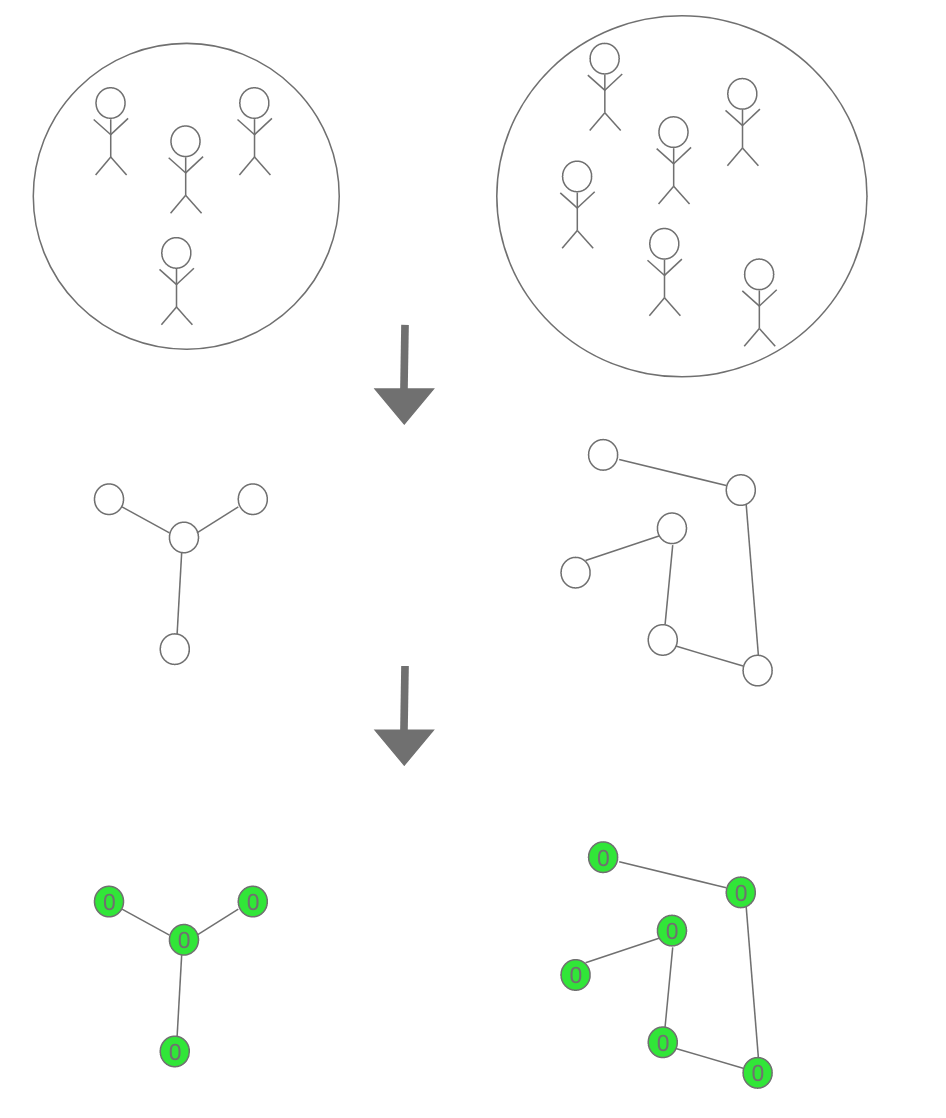
\includegraphics[width=0.5\textwidth]{res/graph_model}
    \caption{Modellierung mit Kontaktnetzwerk}
    \label{fig:graph_model}
\end{figure}

\newpage

\subsection{Erkennung von Infektionen}

\begin{wrapfigure}{R}{0.5\textwidth}
    \centering
    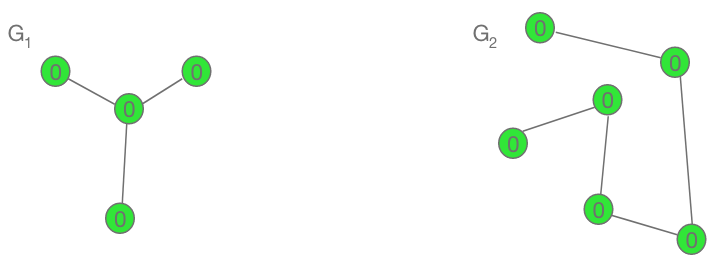
\includegraphics[width=0.4\textwidth]{res/detection_setup}
    \caption{Kontaktnetzwerk}
    \label{fig:detection_setup}
\end{wrapfigure}


Im Folgenden sei $G=(V_1 \cup V_2, E_1 \cup E_2)$ ein Kontaktnetzwerk, welches aus den Zusammenhangskomponenten $G_1=(V_1, E_1)$ und $G_2=(V_2, E_2)$ besteht (siehe \ref{fig:detection_setup})
Sobald ein Kontaktnetzwerk aufgebaut wurde müssen die zugehörigen Personen bestätigte Infektionen melden. Sei $v \in V_1$ der korrespondierende Knoten der infizierten Person $\hat{v}$. Per Definition gilt somit: 
$f(v) = -1$. Ähnlich wie bereits in Abbildung \ref{fig:inf_chain} verdeutlicht kann das Aussetzen einer frühzeitigen Erkennung und Benachrichtigung aller Kontaktpersonen von $\hat{v}$ fatale Folgen haben. Es reicht aus, dass einer der Personen aus $G_1$ zu einer Person aus $G_2$ Kontakt hat, um die Infektionskette rasant wachsen zu lassen:

\begin{figure}[h]
    \centering
    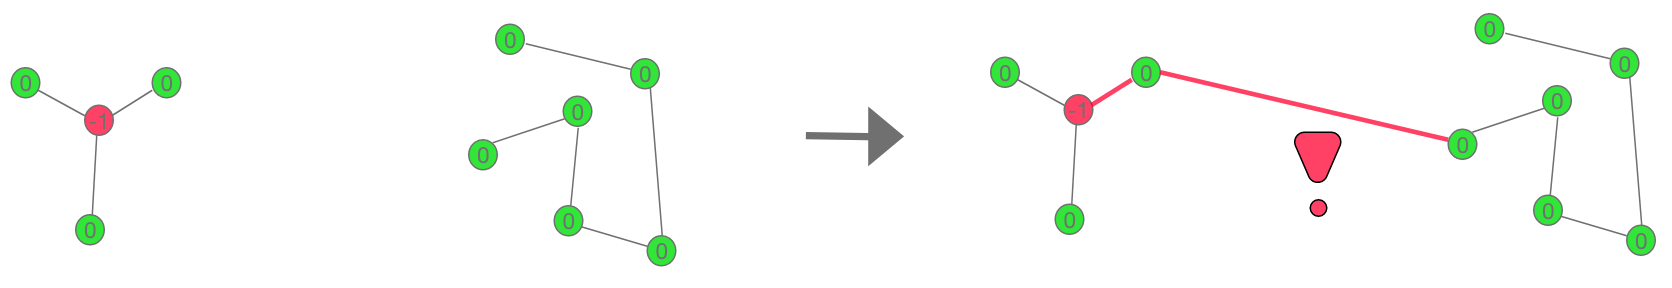
\includegraphics[width=\textwidth]{res/detection_infected}
    \caption{Gefahr bei nicht Erkennung}
    \label{fig:detection_infected}
\end{figure}

Handeln wir jedoch proaktiv und informieren frühzeitig alle Knoten in der Zusammenhangskomponente $G_1$ über eine potentielle Infektion, so können alle korrespondierenden Personen rechtzeitig reagieren und sich in Quarantäne begeben, um so die Infektionskette zu brechen. In unserem Modell setzen wir hierzu
\[f(v') = 1, \forall v' \in V_1 \setminus \{v\}\]

\begin{figure}[h]
    \centering
    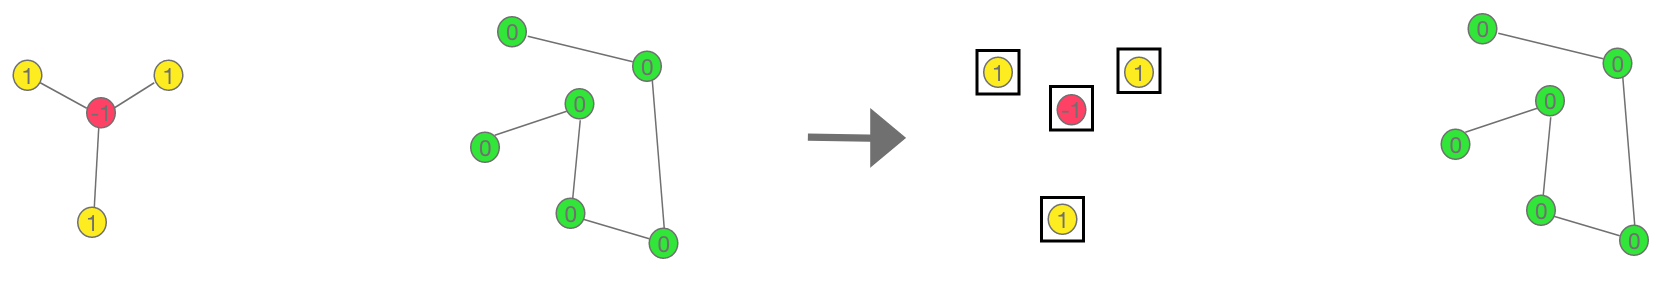
\includegraphics[width=\textwidth]{res/detection_proactive}
    \caption{Eindämmung der Infektionskette}
    \label{fig:detection_infected}
\end{figure}

\paragraph{Algorithmus} Infektionserkennung
---- TODO

\subsection{Prävention von Infektionen}
Während wir mithilfe von Infektionserkennung versuchen wollen die Infektionskette zu brechen, können wir noch proaktiver sein und versuchen die Folgen einer hypothetischen Infektion zu minimieren, indem wir Gelenkpunkte in Zusammenhangskomponenten präventiv unter Quarantäne setzen. 

\paragraph{Definition} Trenner
\\
Es seien $G=(V,E)$ ein einfacher Graph und $A,B \subset V$. Wir bezeichnen $Z=(X,Y$ mit $X \subseteq V$ und $Y \subseteq E$ als $A$-$B$-Trenner, falls jeder $A$-$B$-Weg mindestens einen Knoten aus $X$ oder eine Kante aus $Y$ enthält. 

\paragraph{Definition} Gelenkpunkt
\\
Sei $v \in V$ ein Knoten, der zwei Knoten aus der selben Zusammenhangskomponente in $G$ trennt. Dann ist $v$ ein Gelenkpunkt von $G$ und entspricht somit dem Trenner $Z=(X,Y)$ mit $X = \{v\}$ und $Y = \emptyset$

Mit der Trennung von Zusammenhangskomponenten durch das Entfernen von Gelenkpunkten bzw. durch den Rat zur Quarantäne an korrespondierende Personen können die Auswirkungen von Infektionen innerhalb der Zusammenhangskomponente drastisch gesenkt werden. In Abbildung \ref{fig:prevention_normal} sehen wir die Auswirkungen einer hypothetischen Infektion in $G_2$: Es kommt zur potentiellen Infektion aller Knoten in der Zusammenhangskomponente.

\begin{figure}[h]
    \centering
    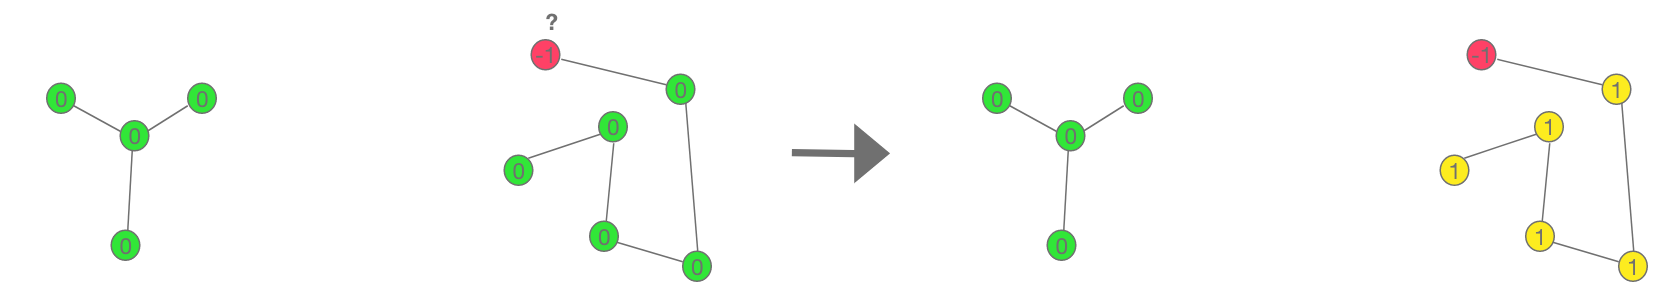
\includegraphics[width=\textwidth]{res/prevention_normal}
    \caption{Auswirkungen ohne Prävention}
    \label{fig:prevention_normal}
\end{figure}

In Abbildung \ref{fig:prevention_proactive} handeln wir allerdings präventiv und setzen den Gelenkpunkt $v$ unter Quarantäne. Eine Infektion in $G_2$ hätte nun wesentlich geringere Auswirkungen:

\begin{figure}[h]
    \centering
    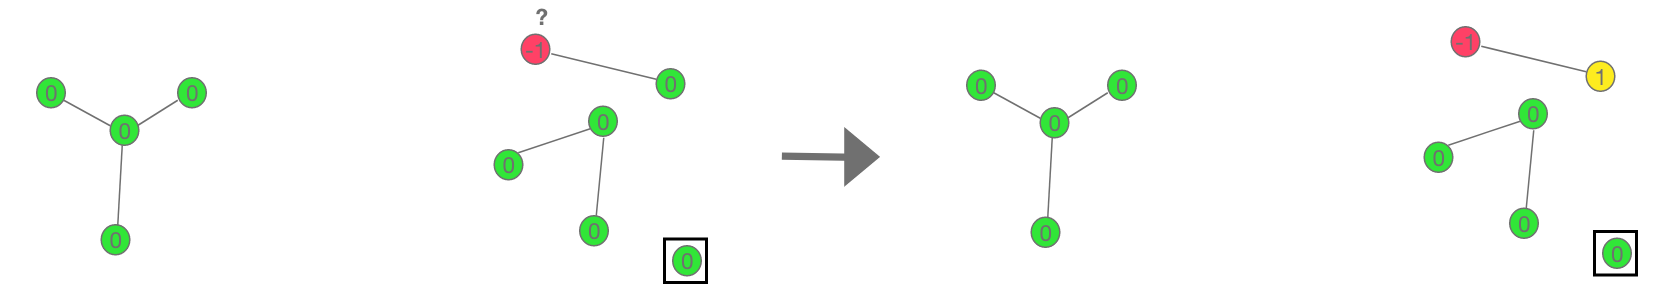
\includegraphics[width=\textwidth]{res/prevention_proactive}
    \caption{Auswirkungen mit Prävention}
    \label{fig:prevention_proactive}
\end{figure}

\paragraph{Algorithmus} Infektionsprävention
---- TODO
\newpage

\section{Implementierung}
Für die Erkennung von Kontakten zwischen Personen $\hat{u}, \hat{v}$ sprich $\hat{u} \leftrightarrow \hat{v}$ beabsichtigen wir ebenfalls von der Bluetooth Technologie auf Smartphones ähnlich wie bei PEPP-PT Gebrauch zu machen. Wir sind uns auch dessen bewusst, dass das Rad nicht neu erfunden werden muss und erhoffen uns daher Kooperationen mit Teams, die in diesem Bereich bereits
Fortschritte erzielt haben. Hierdurch erreichen wir eine hohe Realisierbarkeit auf der Seite des Anwenders.
Ein weiterer wichtiger Faktor für die Realisierbarkeit, Effektivität und Aktualität ist eine angemessene Benutzeroberfläche. Da wir Smartphones nutzen wollen sprechen wir daher von einer benutzerfreundlichen, mobilen Applikation. Die Installation der App wird wahrscheinlich auf freiwilliger Basis hinauslaufen. Weil für die Effektivität und Aktualität der Großteil der Bevölkerung von der App Gebrauch machen muss, ist die Benutzerfreundlichkeit kritisch. Die kontinuierlich gesammelten Kontaktdaten werden nun von der App der Benutzer an einen zentralen Server gesendet. Dort werden sie unserem formalen Graphenmodell entsprech­end modelliert und mithilfe von formalen Methoden und Algorithmen wird das Modell kontinuierlich auf potentielle Infektionen analysiert. Auch hier ist es kritisch, dass
neu erkannte und ärztlich bestätigte Infektionen frühzeitig über die App registriert werden, damit das System korrekt arbeitet. Wird ein Knoten im Graphen als potentiell infiziert eingestuft, so wird die korrespondierende Person unverzüglich informiert.

\subsection{Architektur}

\begin{figure}[H]
    \centering
    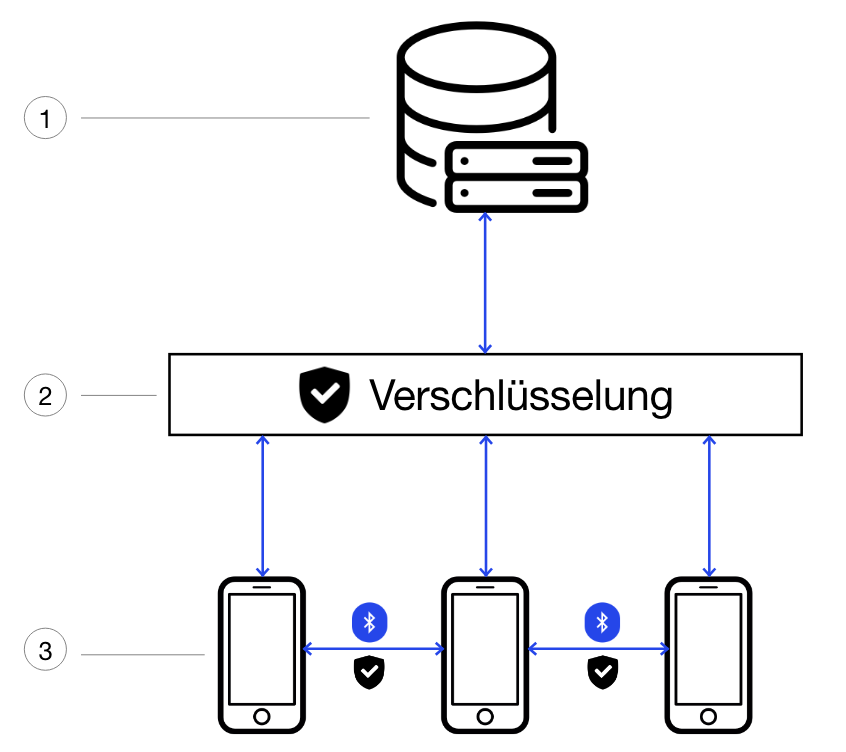
\includegraphics[width=0.7\textwidth]{res/architecture}
    \caption{Architektur}
    \label{fig:architecture}
\end{figure}

%---------------------------------------------------------------------
\begin{thebibliography}{00}
%\bibitem{1}  {\sc Nayfeh,  A.H.} -
% {\it Peturbation Methods.}, John Wiley and Sons, 1976, New York.
%
%\bibitem{2}  {\sc Poincaré, H.} -
%{\it New Methods of celestialmechanics}, Vol. I-III,NASA TTF-450,1967.
%
%\bibitem{3}  {\sc Bauer,H.F.} - {\it  Nonlinear Response of elastic Plates to Pulse Excitations}, J. Appl.Mech., 35, 47-52, 1968.
\end{thebibliography}

%---------------------------------------------------------------------
%\bibliographystyle{sbc}
%\bibliography{sbc-template}

\end{document}
